\documentclass[openany]{article}

%Standard Stefanos Packages
\usepackage[utf8]{inputenc}
\usepackage{dirtytalk}
\usepackage{amsmath}
\usepackage{mathtools}  
\mathtoolsset{showonlyrefs} 
\usepackage{graphicx}
\usepackage{mdframed}
\usepackage{lipsum}
\usepackage{cancel}
\usepackage{systeme}
\usepackage{pgfplots}
\usepackage{textcomp}
\usepackage{geometry}
\usetikzlibrary{arrows}
\geometry{a4paper}
\graphicspath{ {./res/} }
\usepackage{float}
\restylefloat{table}
\newcommand{\comment}[1]{%
	\text{\phantom{(#1)}} \tag{#1}
}
\title{\line(1,0){450}\\ About Internet's Free speech dystopia \\ \large{And how the inability of our law system brings chaos to our internet lifes}  \\\line(1,0){450} \\CS3SC17 - Social, Legal and Ethical Aspects of Computing }
\usepackage{pgfplots}
\author{Stefanos Stefanou}
\newmdtheoremenv{note}{Note}
\pgfplotsset{compat=1.17}

%Extra Packages
\usepackage{tikz}
\usetikzlibrary{automata,positioning}

\usepackage{listings}
\usepackage{xcolor}

\definecolor{dkgreen}{rgb}{0,0.6,0}
\definecolor{gray}{rgb}{0.5,0.5,0.5}
\definecolor{mauve}{rgb}{0.58,0,0.82}

\lstdefinestyle{myScalastyle}{
	frame=tb,
	language=scala,
	aboveskip=3mm,
	belowskip=3mm,
	showstringspaces=false,
	columns=flexible,
	basicstyle={\small\ttfamily},
	numbers=none,
	numberstyle=\tiny\color{gray},
	keywordstyle=\color{blue},
	commentstyle=\color{dkgreen},
	stringstyle=\color{mauve},
	frame=single,
	breaklines=true,
	breakatwhitespace=true,
	tabsize=3,
}
\begin{document}
	\maketitle
	\pagebreak
	
	\section*{Abstract}
	
		The following article, is an attemt to explain the reasons behind the current situation of the internet, in terms of misinformation
		and toxicity. We will present a variety of reasons that compose the problem, and we will argue the need for government regulation and
		intervetion to stabilise our internet lifes
		
	\section*{Introduction}		
		There is a huge discussion lately\cite{Disqussion-about-censorship-1,Disqussion-about-censorship-2} about the social media's 
		attempt to control what has allowed and what is not in their respective platforms. Some argue that this affects the foundations 
		of free speech and narrows down political diversity\cite{dystopians-1},	where others promote stricter censorship 
		in light of out of control incidents\cite{out-of-control}. The situation above may be seen, at first, as a freedom of expression issue, 
		but we will find out that strict social media policies are one of the symptoms of a greater problem. To put it another way, 
		those policies are the cough, where the deeper problem that we will analyze in this report is the flu that our internet society is suffering from.
	\section{Free speech and the internet}
	\subsection*{Setting up the scene}
		We will start with a brief explanation of the current Law regarding content on world wide web platforms. We will refer mostly
		directly to US law for two good reasons. Firstly due to brexit, the EU/UK law is subject to change, meaning that if we claim anything here, 
		this article will be quicly outdated, and Secondly, the law articles that we will present here will still align with EU/UK law in some degree.
		We still may refer to EU/UK law when the given law will be completely unaffected from brexit.
	\subsection*{About free speech}
		The principle of free speech is, without a dought, one of the most important fruits of democracies. It is a fundamental right that 
		makes societies to flourish. In recent times, there is much speculation around the topic, and many feel that 'Free speech' 
		is at risk. But what is 'Free speech'? Under UK Law, The Human Rights Act of 1998\cite{human-rights-act} States that everyone has the right to 
		freedom of expression". But the Law also states that this freedom "may be subject to formalities, conditions, restrictions or penalties 
		as are described by Law and are necessary for a democratic society". In essence, the government has an obligation to guarantee your 
		freedom of 'expression' as long as you honor the necessary conditions. This is the case because as a citizen of the country, it is 
		essential to follow some rules, to follow the Law. It is not possible to structure a democratic and fair society without laws. It is important
		to note the difference between 'Free Speech' and something that i would like to call, 'Chaotic Speech'. Free Speech doesnt mean 'i can say whatever
		i want'. There are exceptions\cite{free-speech-eu,free-speech-uk,free-speech-us}, and everybody needs to be aware of that.
	\subsection*{Unacountability on the internet}
		Social Life on the internet, on the other hand, is problematic when it comes to the implementation of 'democratic and fair society'. 
		The very nature of the internet makes it structurally immune (to some degree) to law enforcement\cite{internet-and-law-enforcement}. 
		Removing the only way to enforce 'fairness' (the Law) makes the internet an anarchist society. Internet from its first days up until 
		today is relatively easy to commit a crime, such as to harass or insult someone and get away with it. Prosecuting 
		people on the internet is a difficult task, and there are none \textit{democratic} governments around the world managed to solve it  yet.
	\subsection*{The explosion of the internet}
		In the first days of all majors social platforms, such as Facebook, Youtube, or Twitter, at the distant 2004-2006, there was almost no content 
		filtering policies. The instances of extremism and violations were few and scattered. This is something to be expected though, given that very 
		few people were on the internet back then, in comparison with todays numbers. No violations, no problem, so no regulations; what could possibly 
		go wrong?
	\begin{figure}[H]
		\iftrue
		\caption{Number of Internet users in years 1993-2014}
		\centering
		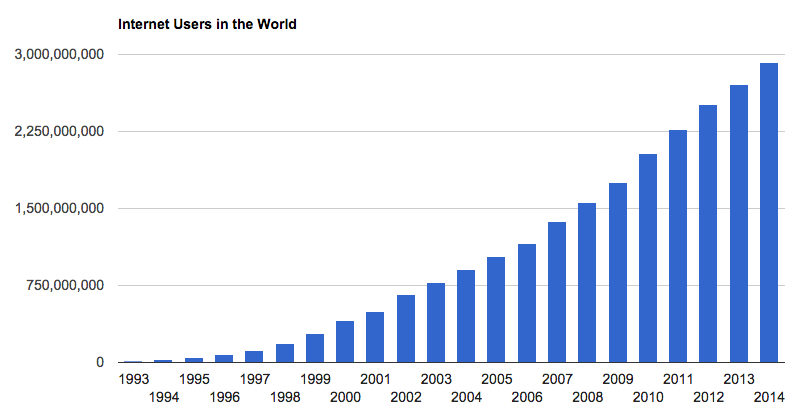
\includegraphics[scale=0.3]{res/users}
		\fi
	\end{figure}
		The internet can be seen as a society, and the societys members are composing the population of that particular society. It is fair 
		to say that as the population increases, the percentage of radical or extremists will remain the same(assuming that everyone is 
		likely probable to have radical views), but the overall number will increase, this is statistically unavoidable. The problem 
		with the extreme behaviors are that very few of them needed are to create problems and disruption. An example of this scenario are the 
		muslim extremists. Those are a tiny minority in the muslim world, but their views and actions are so extreme so they create 
		dirsuption to society.
	\section{The human psycology factor}
	\subsection*{Law landscape}
		According to US Law Section 230\cite{S230} a commercial online platform may fall to 2 distinct categories, Publisher and Public Forum. 
		The main difference in those two categories falls to the legal viability of each for the content that is posted and available in their services. 
		A publisher has the exclusive right to upload content into its platform and is legally responsible for that content. 
		An example of a publisher is the famous newspaper 'Daily Mail'. Daily Mail chooses the articles and the content that is uploaded in its platform 
		and is liable for any possible illegal content. On the other hand, a public forum is a platform that the information has become available 
		through users, and not the company itself; as a consequence, the company is not legally responsible on the content in its services. 
		This is something sensible given that a public forum contents are not directly associated with the company that runs the public forum, 
		but with the users that use this platform on a daily basis. Some public forum examples are Youtube, Facebook, Twitter, etc.
	\subsection*{Public Forums Business Model}
		We need to understand that social media are commercial platforms, usually offering marketing services. Their product is their users. 
		An army of very talented software engineers, marketing specialists, and designers are working around the clock to gain for their respective 
		platform, even more users. Users are not the only metric, though; for the best results, users should be exposed to the platforms mentioned 
		above as much as possible. It is a fact that social media tend to be designed to be as addictive as possible\cite{social-media-addictive-1,
			social-media-addictive-2}. This is something expected under fair market competition; a company wants to earn more!. 
		An unwanted side effect of this if the content on the platforms are affected by this trend. 
	\subsubsection*{The human phycology}
		A very interesting study\cite{emotional-tweets} showed that tweets that contained emotional language were far more likely to become viral 
		and seen by a lot of people than their non-emotional counterparts. Radical and extreme content are almost always emotional-oriented and not 
		fact-based neutral one. The study suggests that human phycology is part of the problem; we are prone to be triggered by something 
		emotional rather than something neutral. This is alarming for the socials media business model. And the reason lies in the technical details...
	\subsubsection*{Antificial Inteligence}
		Artificial intelligence principles have found a great application on social media, especial in the optimization
		on keeping the users as much as possible on the platform, by showing the content that seems that keeps them the most\cite{dark-ai}
		This is something that wasn't a problem in the early days of the internet. Given the target of 'keeping the users as much as possible 
		in the platform' and the fact that emotional content is far more likely to be seen by a lot of people than the neutral counterparts; 
		it is not a surprise that the social media algorithms are pushing radical and extreme behaviour\cite{youtube-radicalize}. This situation
		has created some very real threats to the continuity of our society. Democracies around the world work using the assumption that the majority of
		their citizens, are well informed, and perform logical and not emotional decisions for their future. If the majority of the todays internet gets 
		radicalized or misinformed, our  democratic system is at risk.
	\section{Exposition of the Problem}
	\subsection*{Fake news propaganda}
		Donald J Trump, 45th president of the United States, used the aforementioned problem\footnote{Not claiming that did it on purpose} of 
		our social media life to gain popularity and convenience people with unchecked facts and fake news\cite{trump}. 
		Fake news is often emotionally-oriented, and given the aforementioned study, emotional information are much more likely to be spreaded out. 
		This mechanism can create a great propaganda machine gun that every dictator out there would love to use. 
	\subsection*{The first direct hit to democracy}
		This huge weakness of our online social life has been exposed multiple times by malicious groups to accomplish
		goals that undermine our day to day lifes. The most notable example of this is the incident of 2016 on United States Federal
		elections, when hackers of Russian origin spreaded misinformation to american citizens\cite{russian-hackers-1,russian-hackers-2,russian-hackers-3}.
		The potential here is huge. If a foreign power has this capability of 'hacking' our opinions, then our future is as dim as ever.
	\section{Unregulated Initiative}
	\subsection*{The twitter's bot purge}
		When things go to the extreme, everyone tends on opposite poles; this is exacly what happened when the situation with the violations, 
		insults, and fake news on social media gone out of control around 2018\cite{twitter-crisis}. Twitter, without any external help or 
		regulation from any official legislative body, facing a sudden drop of its users because of the insults and the toxicity that occurred in the 
		platform, started to massively close/ban accounts, that according to twitters policy, were 'responsible' for that content. 
		The problem was that in multiple occurrences, a lot of innocent people that expressed their opinion on a hot topic banned\cite{bot-purge} 
		also from the platform. This situation is not a result of an algorithmic error of Twitter but part of twitters policy. Many voices on 
		the internet were silenced as a result, starting a hot debate around free speech that continues to this day. Let me make this clear, 
		a private company's policy affects the free speech of citizens of all the governments on the planet. If this isn't shockingly alarming, 
		then what is it? Twitter is not the only occasion of false positives  because of bad company policies, Youtube\cite{prageru-youtube} 
		and Facebook\cite{facebook-censor} have also silenced groups falsely under the umbrella of 'extremism'.It is common theme for social 
		media companies to suppress or handle unfavorably groups or specific ideologies, such as conservatives\cite{prageru-youtube}. 
		With the excuse of fairness, companies promote their favorable views and suppress others.
	
	\section{The need for a law system re-design}
		The problem is rather obvious; the judiciary system has left public forums alone to solve the problem of the internet on their own, 
		to act as publishers and control what information is to be seen by millions of people using arbitrary policies and procedures; 
		the effort is undermined because of the very nature of the business model of the respective companies, people are affected in malicious 
		ways due to the inherited human phycology, and there are no law-enforcement bodies to stop this, leading to nothing but chaos\cite{murray}.
		There is a great number of factors that result in this situation. A simple visualization is given below.
	\begin{figure}[H]
		\iftrue
		\caption{Factors Visualisation}
		\centering
		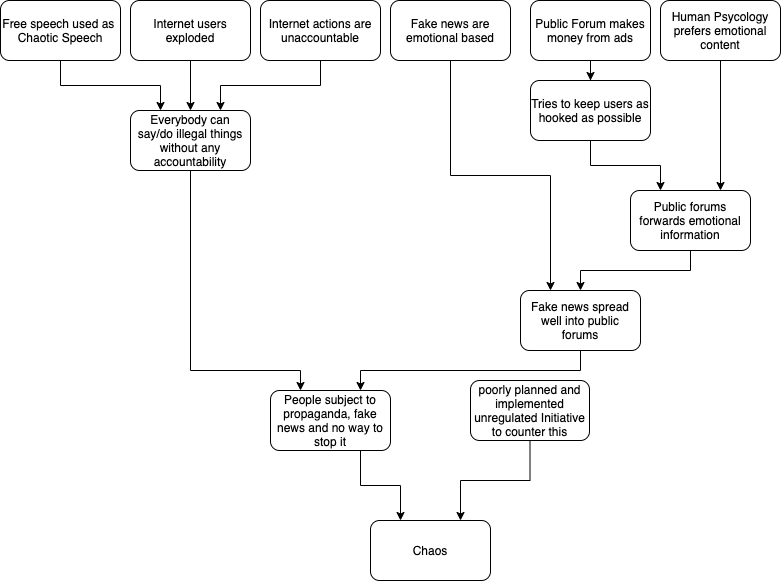
\includegraphics[scale=0.3]{res/nutshell}
		\fi
	\end{figure}
		Our justice system is clearly incapable of handling the situation as it is, and as long this is not changed, the problem will become bigger 
		until, unavoidably, the wrong president will be elected in some part of the world(or maybe is is already been done?). It is really nessesary 
		to wait untill something bad happends before we act? Isnt it obvious that we need a major redesign of our judiciary system?. 
		The structure of the judicial system in many countries has basically remained the same since the enlightenment, is clearly outdated for todays 
		fast-paced online world. Everyone needs to be accountable for his online presence, and face consequences when necessary, The Law needs to step in and restore the order; 
		we cant let private companies handle such important issues. Companies are legal entities with profit in mind, and we cant think only the 
		profits when the discussion comes in matters that affect national security, and probably our society as a whole. When the lesson will be 
		learned?.
	
	
	%Avoid "I" or "We" - write objectively (except in reflections).
	
	\section*{Reflection}
		
		
		CS3SC17 Was one of the most interesting courses of this semester for a number of reasons. Ethics helped me to redefine what's right and what's wrong, 
		improving my internal checks and balances, exposing myself to the theory of ethics and the multiple ethical frameworks that exist out there unlocked 
		a huge improvement potential for me. Law made me understand just how complicated our societies are, and how much in need we were for good laws. 
		I was totally unaware of their real value, and i was discrediting them before that course; this part helped a lot. I remember in one of the first 
		lectures that 'Some programmers are not even aware of the usefulness of laws' and I was clearly one of them. I am very glad that this huge field is 
		available now for me for further study, especially ethics, as in some sense, I can draw lessons from my personal development.
		
		
		The group assessment was a challenge for me because it was pretty unorthodox for the standards of the university; I needed to study a lot about 
		ethics and Law, in order to be able to detect the various issues involving our selected movie; it was a nice challenge that put my aforementioned 
		knowledge with my critical judgment into action. I wasn't just forced to apply textbook knowledge 'dumb-ly,' and I am very grateful for this. 
		The fact that this was group coursework gave me the opportunity to argue for my beliefs, to convince and to be convinced me to blend my 
		knowledge and, most importantly, my critical ability with others and produce a nice result. I am very happy with my team as everyone was 
		greatly prepared and well organized for this. I think that we produced a nice result.
		
		
		In the final coursework, I had the chance to do my first great research on a topic. 27 references, ten videos, three academic papers, and 
		one podcast later, I had formed an opinion about the reasons about todays internet situation, and the need for a legislative body intervention 
		in order to restore order. I wrote and rewrote multiple times parts of this coursework, as I argued internally about various topics, and new 
		findings from my research contradicted my old beliefs. This inductive process of finding the truth was amazing to me, and shielded me from 
		any form of fake news. Now I have the techniques and the ways to find the truth, and this coursework was essential to gain the skills necessary. 
		This course taught me something that I needed a lot; it taught me how to learn and how to do research properly. It taught me ethics and the 
		useability of Law. The course structure had the right amount of explanation and not-explaining something, in order to search it later on my own 
		and further my knowledge. It had the right mix of 'straightforwardness' and difficulty.    
		
	\pagebreak
		\begin{thebibliography}{1}	
			\bibitem{free-speech-us}
			\textit{En.wikipedia.org. 2021. United States Free Speech Exceptions. [online] Available at: <https://en.wikipedia.org/wiki/United\_States\_free\_speech\_exceptions> [Accessed 10 January 2021].}

			\bibitem{free-speech-uk}
			\textit{En.wikipedia.org. 2021. Censorship In The United Kingdom. [online] Available at: <https://en.wikipedia.org/wiki/Censorship\_in\_the\_United\_Kingdom> [Accessed 10 January 2021].}
			
			\bibitem{free-speech-eu}
			\textit{European Union Agency for Fundamental Rights. 2021. Article 11 - Freedom Of Expression And Information. [online] Available at: <https://fra.europa.eu/en/eu-charter/article/11-freedom-expression-and-information> [Accessed 10 January 2021].}
			

			\bibitem{murray}
			\textit{En.wikipedia.org. 2020. Murray-Hill Riot. [online] Available at: <https://en.wikipedia.org/wiki/Murray-Hill\_riot> [Accessed 10 December 2020].}
			
			\bibitem{trump}
			\textit{BBC News. 2020. How 'Fake News' Entered The Mainstream. [online] Available at: <https://www.bbc.com/news/av/world-us-canada-46175024> [Accessed 10 December 2020].}
			
			
			\bibitem{russian-hackers-1}
			\textit{the Guardian. 2020. Russian Hackers Targeting US Political Campaigns Ahead Of Elections, Microsoft Warns. [online] Available at: <https://www.theguardian.com/technology/2020/sep/10/microsoft-russia-us-election-2020-hackers> [Accessed 10 December 2020].}
			
			\bibitem{russian-hackers-2}
			\textit{Nytimes.com. 2020. Russian Hacking And Influence In The U.S. Election. [online] Available at: <https://www.nytimes.com/news-event/russian-election-hacking> [Accessed 10 December 2020].}
			
			\bibitem{russian-hackers-3}
			\textit{(www.dw.com), D., 2020. Russia, Iran Meddling With US Elections: 'Hacking Of Our Hearts And Minds' | DW | 31.10.2020. [online] DW.COM. Available at: <https://www.dw.com/en/russia-iran-meddling-with-us-elections-hacking-of-our-hearts-and-minds/a-55454124> [Accessed 10 December 2020].}
			
			\bibitem{prageru-youtube}
			\textit{Cdn.ca9.uscourts.gov. 2020. [online] Available at: <https://cdn.ca9.uscourts.gov/datastore/opinions/2020/02/26/18-15712.pdf> [Accessed 10 December 2020].}
			
			\bibitem{bot-purge}
			\textit{Medium. 2020. Twitter’S Suspension Bots Are Out Of Control. [online] Available at: <https://onezero.medium.com/the-upgrade-5a5cc79fc9bb> [Accessed 10 December 2020].}
			
			
			\bibitem{dark-ai}
			\textit{Datascience at home podcast. 2020. The Dark Side Of AI: Social Media And The Optimization Of Addiction. [online] Available at: <https://datascienceathome.com/the-dark-side-of-ai-social-media-and-the-optimization-of-addiction/> [Accessed 10 December 2020].}
			
			
			\bibitem{emotional-tweets}
			\textit{Tago, Kiichi \& Jin, Qun. (2018). Influence analysis of emotional behaviors and user relationships based on Twitter data. Tsinghua Science and Technology. 23. 104-113. 10.26599/TST.2018.9010012. }
			
			\bibitem{twitter-crisis}
			\textit{Fast Company. 2020. “Did We Create This Monster?” How Twitter Turned Toxic. [online] Available at: <https://www.fastcompany.com/40547818/did-we-create-this-monster-how-twitter-turned-toxic> [Accessed 10 December 2020].}		
			
			
			\bibitem{social-media-addictive-1}
			\textit{BBC News. 2020. Social Media Apps Are 'Deliberately' Addictive To Users. [online] Available at: <https://www.bbc.com/news/technology-44640959> [Accessed 10 December 2020].}		
			
			
			\bibitem{social-media-addictive-2}
			\textit{Business Insider. 2020. Instagram And Facebook Are Intentionally Conditioning You To Treat Your Phone Like A Drug. [online] Available at: <https://www.businessinsider.com/facebook-has-been-deliberately-designed-to-mimic-addictive-painkillers-2018-12?r=US\&IR=T> [Accessed 10 December 2020].}		
			
			
			
			\bibitem{internet-and-law-enforcement}
			\textit{TechRepublic. 2020. What Makes Cybercrime Laws So Difficult To Enforce. [online] Available at: <https://www.techrepublic.com/blog/it-security/what-makes-cybercrime-laws-so-difficult-to-enforce/> [Accessed 10 December 2020].}			
			\bibitem{human-rights-act}
			\textit{Human Rights Act 1998.}			
			\bibitem{Disqussion-about-censorship-1}
			\textit{Koetsier, J., 2020. Social Censorship: Should Social Media’S Policy Be Free Speech?. [online] Forbes. Available at: <https://www.forbes.com/sites/johnkoetsier/2020/10/25/social-censorship-should-social-medias-policy-be-free-speech/?sh=34ed5860489a> [Accessed 10 December 2020].}
			\bibitem{Disqussion-about-censorship-2}
			\textit{Yaraghi, N., 2020. Regulating Free Speech On Social Media Is Dangerous And Futile. [online] Brookings. Available at: <https://www.brookings.edu/blog/techtank/2018/09/21/regulating-free-speech-on-social-media-is-dangerous-and-futile/> [Accessed 10 December 2020].}
			\bibitem{out-of-control}
			\textit{Amnesty.org. 2020. Toxic Twitter - Triggers Of Violence And Abuse Against Women On Twitter. [online] Available at: <https://www.amnesty.org/en/latest/research/2018/03/online-violence-against-women-chapter-2/> [Accessed 10 December 2020].}
			\bibitem{dystopians-1}
			\textit{Jr., D., 2020. Free Speech Or Censorship? Social Media Litigation Is A Hot Legal Battleground. [online] ABA Journal. Available at: <https://www.abajournal.com/magazine/article/social-clashes-digital-free-speech> [Accessed 10 December 2020].}
			\bibitem{Disqussion-1}
			\textit{How to Adapt Regulatory Framework to the Digital Age?  (2017) INTERNAL MARKET AND CONSUMER PROTECTION COMMITEE-European Parliament.}
			\bibitem{Disqussion-2}
			\textit{Reform of the EU liability regime for online intermediaries (2020) European Parliamentary Research Service, Tambiama Madieg.}
			\bibitem{A14}
			\textit{Eur-lex.europa.eu. 2000. DIRECTIVE 2000/31/EC OF THE EUROPEAN PARLIAMENT AND OF THE COUNCIL. [online] Available at: <https://eur-lex.europa.eu/legal-content/EN/TXT/PDF/?uri=CELEX:32000L0031\&from=EN> [Accessed 9 December 2020].}
			\bibitem{S230}
			\textit{Eur-lex.europa.eu. 2000. DIRECTIVE 2000/31/EC OF THE EUROPEAN PARLIAMENT AND OF THE COUNCIL. [online] Available at: <https://eur-lex.europa.eu/legal-content/EN/TXT/PDF/?uri=CELEX:32000L0031\&from=EN> [Accessed 9 December 2020].}
			\bibitem{youtube-radicalize}
			\textit{The Conversation. 2020. Youtube's Algorithms Might Radicalise People – But The Real Problem Is We've No Idea How They Work. [online] Available at: <https://theconversation.com/youtubes-algorithms-might-radicalise-people-but-the-real-problem-is-weve-no-idea-how-they-work-129955> [Accessed 10 December 2020].}
			\bibitem{facebook-censor}
			\textit{En.wikipedia.org. 2020. Criticism Of Facebook. [online] Available at: <https://en.wikipedia.org/wiki/Criticism\_of\_Facebook\#Kurdish\_opposition\_censorship> [Accessed 10 December 2020].}
			
		\end{thebibliography}
\end{document}